\documentclass[tikz,border=10pt,12pt]{standalone}
% Shared preamble for standalone-compiled dc_paper figures.
% Copies just the bits of dc_paper.tex's preamble that figures need.

\usepackage{amsmath,amssymb,amsthm,mathtools,bm}
\usepackage{siunitx}
\sisetup{detect-all,group-separator={,},per-mode=symbol}

\usepackage[T1]{fontenc}
\usepackage{xcolor}
\usepackage{enumitem}
\usepackage{mathpazo}                % Palatino body + matching math
\usepackage[scaled=0.92]{helvet}     % Helvetica sans
\usepackage{courier}                 % monospace
\usepackage{microtype}

% --- IA brand colour palette (must match dc_paper.tex) ---
\definecolor{iadark}{HTML}{1B1815}
\definecolor{iabone}{HTML}{FAFAF7}
\definecolor{iaaccent}{HTML}{A04A1F}
\definecolor{iataupe}{HTML}{F2EDE6}
\definecolor{iarule}{HTML}{3A332D}
\definecolor{iagrey}{HTML}{5A524A}

% --- graphics ---
\usepackage{tikz}
\usepackage{circuitikz}
\usepackage{pgfplots}
\pgfplotsset{compat=1.18}
\usetikzlibrary{arrows.meta,positioning,shapes.geometric,calc,fit,
                decorations.pathreplacing,decorations.markings,
                shadows.blur,backgrounds}

% --- math macros from dc_paper.tex preamble (figures use them) ---
\newcommand{\E}{\mathbb{E}}
\newcommand{\Var}{\operatorname{Var}}
\newcommand{\Cov}{\operatorname{Cov}}
\newcommand{\Cor}{\operatorname{Cor}}
\newcommand{\Prb}{\mathbb{P}}
\newcommand{\R}{\mathbb{R}}
\newcommand{\N}{\mathbb{N}}
\newcommand{\1}{\mathbf{1}}
\newcommand{\VaR}{\operatorname{VaR}}
\newcommand{\TVaR}{\operatorname{TVaR}}
\newcommand{\ES}{\operatorname{ES}}
\newcommand{\dd}{\mathrm{d}}
\newcommand{\given}{\,\vert\,}
\newcommand{\set}[1]{\left\{#1\right\}}
\newcommand{\norm}[1]{\left\Vert #1 \right\Vert}
\DeclareMathOperator*{\argmin}{arg\,min}
\DeclareMathOperator*{\argmax}{arg\,max}

% \textwidth has no meaning in standalone class; give it a value matching
% the paper's A4 + 1-inch margins so any leftover \resizebox{\textwidth}
% gracefully sizes the figure to that nominal width.
\setlength{\textwidth}{15.92cm}

\begin{document}
\pagecolor{iabone}
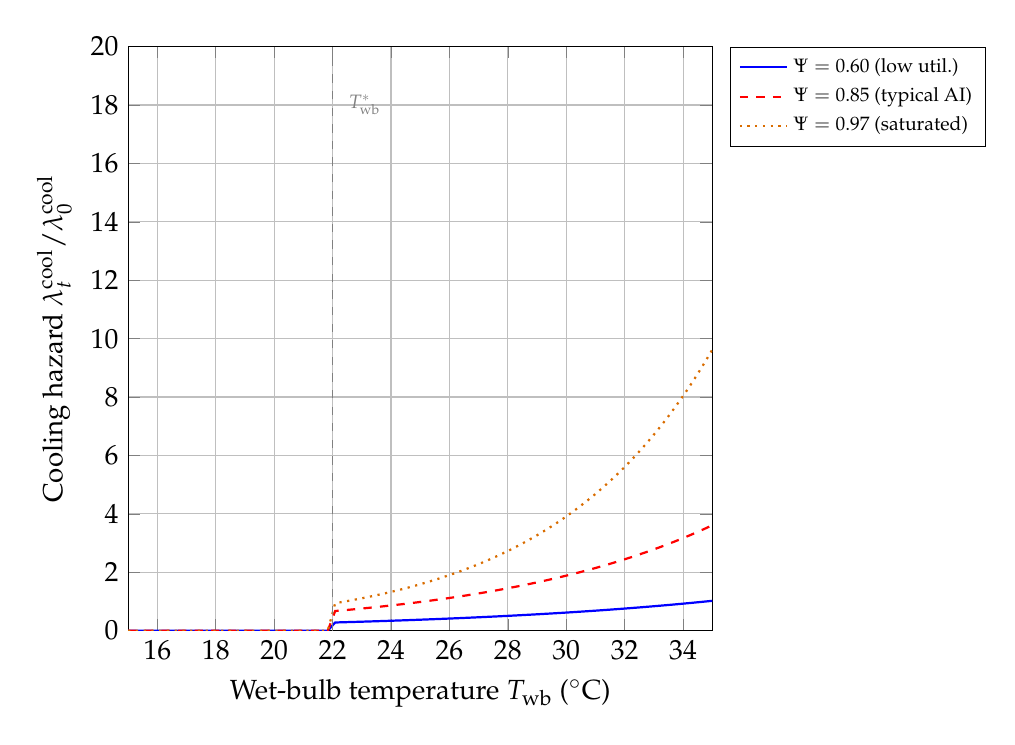
\begin{tikzpicture}
\begin{axis}[
   width=9cm, height=9cm,
   xlabel={Wet-bulb temperature $T_{\mathrm{wb}}$ ($^\circ$C)},
   ylabel={Cooling hazard $\lambda^{\mathrm{cool}}_t/\lambda^{\mathrm{cool}}_0$},
   xmin=15, xmax=35, ymin=0, ymax=20,
   grid=major,
   legend pos=outer north east,
   legend cell align=left,
   legend style={font=\scriptsize}
]
% Three Psi (utilisation) levels
\addplot[blue,thick,domain=15:35,samples=80]
   {(x>22) * 0.6^2.5 * exp(0.10*(x-22))};
\addlegendentry{$\Psi=0.60$ (low util.)}
\addplot[red,thick,dashed,domain=15:35,samples=80]
   {(x>22) * 0.85^2.5 * exp(0.13*(x-22))};
\addlegendentry{$\Psi=0.85$ (typical AI)}
\addplot[orange!85!black,thick,dotted,domain=15:35,samples=80]
   {(x>22) * 0.97^2.5 * exp(0.18*(x-22))};
\addlegendentry{$\Psi=0.97$ (saturated)}
% design wet-bulb threshold
\draw[gray,dashed] (axis cs:22,0) -- (axis cs:22,20);
\node[gray,font=\scriptsize] at (axis cs:23.1,18) {$T^*_{\mathrm{wb}}$};
\end{axis}
\end{tikzpicture}
\end{document}
